%!TEX root = ../dissertation.tex

\chapter{Knowledge Enhanced Neural Networks}\label{chapt:2}
Knowledge Enhanced Neural Network (KENN) is a special type of model; more specifically, is a residual layer designed to by attached at the end of a standard Neural Network (NN), in order to boost its predictive performances via the addition of a Prior Knowledge, in the form of First Order Logic (FOL) clauses.

\section{Theoretical Framework}\label{sec:theoretical_framework}
 We present here the theoretical framework behind KENN. The first step will be to rigorously define the symbolic language and how to link it with the theoretical framework of NNs, which consists in defining a semantic for the language. Next, we will describe the process with which the truth value of a clause can be increased, and how to integrate this method inside NNs.
 
 \subsection{Prior Knowledge and language semantic}

\begin{definition}[Prior Knowledge]
	Collection of formulas of a function-free FO language $\mathcal{L}$ whose signature is defined with a set of constants $\mathcal{C} = \{a_1, \dots, a_l\}$ and a set of predicates $\mathcal{P} = \{p_1, \dots, p_q\}$. Each predicate can be applied to a specific number of constants $n$, which we will define as the \textit{arity} of the predicate.
\end{definition}

\begin{definition}[Clause]
	A clause is defined to be of the following form:
	\begin{equation}
	c := \bigvee_{i=1}^k l_i, \quad l_i \neq l_j \quad \forall i \neq j.
	\end{equation}
	where $l_i$ is a literal, i.e. a formula constituted only by a $n$-ary predicate, or its negation. Also clauses have an arity, which is by definition the maximum arity of the predicates that constitute it.
\end{definition}

One example of a clause could be the following: 
\begin{equation}
c(x,y) = \neg Smoker(x) \vee \neg Friends(x,y) \vee Smoker(y)
\label{example:clause}
\end{equation} which is equivalent to the clause $Smoker(x) \wedge Friends(x,y) \Rightarrow Smoker(y)$, but expressed as a disjunction of literals. Such a clause is constituted by two predicates: $Smoker(x)$, a unary predicate expressing the statement \say{\textit{$x$ is a smoker}}, and $Friends(x,y)$, a binary predicate which expresses the statement \say{\textit{$x$ and $y$ are friends}}. Therefore, this clause expresses the rule \say{\textit{if $x$ is a smoker and $x$ and $y$ are friends, than also $y$ is a smoker}}. Note that the variables $x$ and $y$ are supposed to be universally quantified, since our aim is to express general knowledge. We now give another definition:

\begin{definition}[Grounding of a clause]
	The grounding of an $n$-ary clause $c$, denoted as \\ $c[x_1/k_1, \dots, x_n/k_n]$,
	is the clause obtained by substituting $k_i$ to $x_i, \forall i=1,\dots,n$.
\end{definition}

Going back to the example of before, assume that $a$ and $b$ are two specific persons. Then, the grounding of clause (~\ref{example:clause}) will be $$c(x/a, y/b) = c(a,b) = \neg Smoker(a) \vee \neg Friends(a,b) \vee Smoker(b).$$

The next step is to build a semantic for the formal language $\mathcal{L}$, that is, how to interpret the symbols that we are working with. In practice, this will consist on defining a way to map constants towards a domain, and predicates to functions that go from such domain to a truth value. To clarify, consider the following example: let $a$ be a constant and let $P$ be a predicate, such that $P(x)$ expresses the statement \say{\textit{$x$ is a prime number}}. In this case, there is a natural way to define an interpretation for our symbols, that is to map constants to the domain of natural numbers and to map $P$ to the function $f: \mathbb{N}\longrightarrow\{0,1\}$, where $f(n)=1$ if $n$ is prime, and $0$ otherwise. Now, we define the semantic of $\mathcal{L}$.

\begin{definition}[Semantic of $\mathcal{L}$]
	The semantic of $\mathcal{L}$ is defined by means of a pair of functions $\left( \mathcal{I}_{\mathcal{C}}, \mathcal{I}_{\mathcal{P}} \right)$, that, together, define an \textit{interpretation} for the symbols of our language and are defined as follows:
	\begin{equation}
	\begin{aligned}[c]
			\mathcal{I}_{\mathcal{C}}: \mathcal{C} &\longrightarrow \mathbb{R}^l\\
			c&\longmapsto x,
	\end{aligned}
	\qquad \qquad
	\begin{aligned}[c]
	\mathcal{I}_{\mathcal{P}}: \mathcal{P} &\longrightarrow \left( \mathbb{R}^{nl} \rightarrow \left[0,1\right] \right)\\
	P &\longmapsto f
	\end{aligned}
	\end{equation}	
	Where $n$ is the arity of the predicate $P$ and $f$ is a function that takes in input the interpretations of $n$ constant symbols, $\mathcal{I}_C(c_1), \dots, \mathcal{I}_C(c_n)$ and returns the truth value of $P(c_1,\dots,c_n)$. Note that, to make the notation lighter, we will omit the subscript when it's clear whether the argument of the interpretation is a literal or a constant term.
\end{definition}

One could already see an analogy with the theoretical setup of NNs. In fact, each constant symbol $c$ is mapped to a $l$-dimensional real vector, which can be seen as the feature vector characterizing the real world object identified by $c$. Another important detail is that the truth value of each literal, in our setup, is not determined by a hard assignment of $0$ or $1$, but is represented by a real number in the interval $\left[ 0,1 \right]$. This is a crucial point: indeed, the truth value in our semantic is trying to represent predictions by a NN, which are always expressed in terms of probability. The natural consequence of this choice is that, from this point on, we will have to rely on the rules of Fuzzy Logic, which is a generalization of the standard Boolean logic where the truth value of variables can take the value of any real number between $0$ and $1$. 

\subsection{$t$-conorm Functions}
With our definition of a semantic for $\mathcal{L}$, we can now give an interpretation for constants and predicates. The next step is to find a way to interpret clauses, or, more specifically, a way to determine the truth value of a grounded clause. We saw that, by definition, a clause is a disjunction of literals: this means that we only need a way to define the interpretation of a negated predicate and of the disjunction of two predicates. As stated above, since we are allowing truth values in the range $\left[ 0,1\right]$, we will need to use the rules of Fuzzy Logic. For computing the truth value of a negated predicate, the standard way in Fuzzy Logic is to use the Lukasiewicz Negation.

\begin{definition}[Lukasiewicz Negation]
	If $P \in \mathcal{P}$ is a predicate, then:
	\begin{equation}
	\mathcal{I}(\neg P) = 1 -\mathcal{I}(P)\footnote{Writing $1 -\mathcal{I}(P)$ is a slight abuse of notation since $\mathcal{I}(P)$ is a function (or is it?).} 
	%TODO: capire se è abuso di notazione 
	\label{eq:lukasiewicz}
	\end{equation}
		
	
\end{definition}

So for example if the truth value of a predicate is $\mathcal{I}(P)(x) = 0.8$, the truth value of its negated copy would be $\mathcal{I}(\neg P)(x) = 0.2$. It is worth noting that this definition is equivalent to the Boolean negation when $\mathcal{I}(P) = 0$ or $\mathcal{I}(P) = 1$.

With this tool we are now able to compute the truth value of any literal. There remains to see how to define the interpretation of a disjunction of literals. To do this, we introduce the concept of $t$-conorm functions.

\begin{definition}[$t$-conorm ]
	A $t$-conorm is a function $\perp: \left[0,1 \right]^2 \rightarrow \left[0,1 \right]$ that satisfies the following properties:
	\begin{enumerate}
		\item $\perp(a, b)=\perp(b, a)$
		\item $\perp(a, b) \leq \perp(c, d)$ if $a \leq c$ and $b \leq d$
		\item $\perp(a, \perp(b, c))=\perp(\perp(a, b), c)$
		\item $\perp(a, 0)=a$
	\end{enumerate}
\end{definition}
By definition, $\perp$ takes values in $\left[0,1 \right]^2$, but can be easily extended to $\left[0,1 \right]^n$ for any $n$, by defining:
\begin{equation*}
\perp(a_1,\dots,a_n) := \perp(a_1,\perp(a_2,\dots \perp(a_{n-1},a_n))).
\end{equation*}
In Fuzzy Logic, $t$-conorm functions are used to represent the concept of logical disjunction, and will be the tool employed to represent the interpretation of a disjunction of literals. Specifically:
\begin{equation}
\mathcal{I}(l_1 \vee \dots \vee l_n) = \perp(\mathcal{I}(l_1),\dots,\mathcal{I}(l_n)).
\end{equation}
It is also worth specifying that $\mathcal{I}(l_1 \vee \dots \vee l_n)$ will be a function from $\mathbb{R}^{nl}$ to $\left[0,1\right]$, where $n$ is the arity of the clause $c := \bigvee_{i=1}^k l_i$.
With the given definitions, we have all that is needed to compute the truth value of any grounded clause. From a practical point of view, the only remaining step would be to choose a specific $t$-conorm function. KENN uses the Gödel $t$-conorm function, which is also known as the Maximum $t$-conorm and is defined as

\begin{equation*}
\perp_{max}(a,b) = \max\{a,b\},
\end{equation*}
which, as above, can be extended like follows:
\begin{equation*}
\perp_{max}(t) = \max_{i=1,\dots,l} t_i, \quad \forall t \in \mathbb{R}^l.
\end{equation*}

We are now finally ready to fully understand how this theoretical framework is able to describe the predictions of a NN. Suppose that we have a dataset $\mathcal{X}=\{x_1, \dots, x_n\}, x_i\in\mathbb{R}^l$, where each $x_i$ belongs to one or more classes $\left( P_1, \dots, P_m \right)$. The task in which the NN must learn to classify each input into one or more output classes is known  in Machine Learning as a multilabel classification problem. To tackle this kind of task, a NN architecture will present, in the last layer, $m$ output units, each of which will be finally subject to a sigmoidal activation function. After training, the NN will have learned to approximate a function $h(x_i) = y_i \in \mathbb{R}^m$, where $(y_i)_j = \mathbb{P}(x_i\text{ belongs to class }j).$ Now, if we consider:
\begin{enumerate}
	\item $\mathcal{P} = \{P_1,\dots,P_m\}$ to be predicates defined as $P_i(x) = $ \say{$x$ belongs to class $P_i$};
	\item $\{x_1,\dots, x_n\}$ to be the interpretations of the constants $\mathcal{C} = \{c_1,\dots,c_n\}$, which represent the real-world objects of our dataset,
\end{enumerate}  it is clear that the entries of $y_i$ can be seen as truth values of the predicates $\{P_1,\dots,P_m\}$. More formally:
\begin{equation}
(y_i)_j = \mathcal{I}_{NN}(P_j)(x_i), \quad \forall i=1,\dots,n, \forall j=1,\dots,m.
\end{equation}
Hence, the whole NN defines an interpretation for each predicate $P_i$, which we denoted as $\mathcal{I}_{NN}$. Therefore, given a clause $c := \bigvee_{i=1}^k l_i$ and given and $\{x_1,\dots,x_d\}$ a collection of feature vectors (where $d$ is the arity of $c$), then the truth value of the grounded clause predicted by the NN will be $\perp(y_c)(x_1,\dots,x_k)$, where:
\begin{equation}
y_c \in \mathbb{R}^k, \quad(y_c)_i = \begin{cases}
\mathcal{I}(l_i) \text{ if } l_i \text{ is not a negated predicate}\\
1-\mathcal{I}(l_i) \text{ otherwise.}
\end{cases}
\end{equation}

The intuition behind KENN is very simple: given $y$ the vector of predictions by the NN, a new layer is added at its end with the aim to modify $y$ and obtain a new vector of predictions $y'$, of the form $y'=y+\delta$, such that $y'$ improves the truth value of each clause present in the base knowledge and, at the same time, keeps the quantity $\|y'-y\|_2$ minimal. It is worth noticing that this new layer introduced by KENN, called Knowledge Enhancer (KE), is a kind of residual layer, since it learns to represent the quantity $\delta = y'-y$.

\subsection{$t$-conorm Boost Functions}
The next problem is to understand how to improve the truth value of a single clause. Since this truth value is represented by a $t$-conorm function, this involves finding a way to let the value of $\perp(y)$ rise by manipulating the value of $y$. To do this, we define a new class of functions.

\begin{definition}[$t$-conorm Boost Function (TBF)]
	A function $\delta:[0,1]^{n} \rightarrow[0,1]^{n}$ is a $t$-conorm Boost Function (TBF) if:
	$$
	0 \leq t_{i}+\delta(t)_{i} \leq 1  \quad \forall n \in \mathbb{N} \quad \forall \mathbf{t} \in[0,1]^{n}.
	$$
	Let $\Delta$ denote the set of all TBFs.
\end{definition}
From the definition follows a simple but essential result.

\begin{lemma}
	Given $\perp$ any $t$-conorm and $\delta \in \Delta$, it holds that:
	$$ \perp(t) \leq \perp(t + \delta(t)).$$
\end{lemma}
\begin{proof}
	By definition of TBF, $\delta(t)_i \geq 0$ and also $t_i \geq 0$. This implies that $$t_i \leq t_i + \delta(t)_i, \quad \forall i=1,\dots,n.$$By the monotonicity of $t$-conorms, it follows that $\perp(t) \leq \perp(t+\delta(t))$.
\end{proof}

The purpose of such TBF $\delta$ is to update the NN predictions $y \in \mathbb{R}^m$ to a new vector %$y'=y+\delta(y)$, 
in such a way that the truth value of each clause increases. The problem is now how to choose such a TBF. It is clear that not all the $\delta \in \Delta$ would be useful: for example, one could choose the function $\delta(y)_i = 1-y_i, \quad \forall i=1,\dots,n$. In this way, we would obtain an updated truth value of $1$ for any clause, independently of $y$. This of course would be pointless, and would render the predictions of the base NN useless. For this reason another requirement for $y'$ is needed. Specifically, as we already mentioned, KENN is built in such a way that the learnt $\delta$ improves the $t$-conorm value in a minimal way. To be more rigorous, we will now formally define the concept of a minimal TBF.

\begin{definition}[Minimal TBF]
	A function $\delta \in \Delta$ is minimal with respect to a norm $\|\cdot\|$ and a $t$-conorm $\perp$ if and only if:
	$$
	\left\|\delta^{\prime}(t)\right\|<\|\delta(t)\| \Rightarrow \perp\left(t+\delta^{\prime}(t)\right)<\perp(t+\delta(t)), \quad \forall \delta^{\prime} \in \Delta, \quad \forall n \in \mathbb{N}, \quad \forall t \in[0,1]^{n}.
	$$
\end{definition}

As mentioned above, KENN works with the Gödel $t$-conorm function and the $L_p$ norm $\|x\|_p = \left( \sum_{i=1}^n |x_i|^p \right)^{\frac{1}{p}}$.
The next step at this point is to find such a minimal TBF. In the following result, we present a possible form that a minimal TBF can assume.

\begin{theorem}
	For any function $f: \mathbb{R}^{n} \rightarrow \mathbb{R}$ we define $\delta^{f}: \mathbb{R}^{n} \rightarrow \mathbb{R}^{n}$ as
	$$
	\delta^{f}(t)_{i}= \begin{cases}f(t) & \text { if } i=\arg\max_{j=1}^n t_{j} \\ 0 & \text { otherwise }\end{cases}
	$$
	Let $f: \left[0,1\right]^{n} \rightarrow \left[0,1\right]$ satisfying $0 \leq f(t) \leq 1- \max_{j=1}^n t_j$. Then, $\delta^f$ is a minimal TBF for the Gödel $t$-conorm function and the $L_p$ norm.
\end{theorem}
\begin{proof}
	$\delta^f$ is a TBF. Indeed $\delta^f(t) \geq 0$ and $0 \leq t_i + \delta^f(t_i) \leq 1$ because $f(t) \leq 1- \max_j t_j$. Therefore we only need to prove that $\delta^f$ is minimal. Take $\delta \in \Delta$, with $\|f(t)\|_p < \|\delta^f(t)\|_p$. We have to show that $$\perp\left(t+\delta\left(t\right)\right) \leq \perp\left(t+\delta^f\left(t\right)\right).$$ 
	Now define $j=\arg\max_k \left(t_k + \delta(t)_k\right)$. By definition of the Gödel $t$-conorm we can immediately derive that:
	\begin{equation}
	\perp(t+\delta(t)) = t_j+\delta(t)_j.
	\label{eq:proof1}
	\end{equation}
	Now, defining $i=\arg\max_k t_k$, using the same reasoning and exploiting the definition of $\delta^f$ it follows that:
	\begin{equation}
	\perp(t+\delta^f(t)) = t_i + f(t).
	\label{eq:proof2}
	\end{equation}
	By combining (\ref{eq:proof1}) and (\ref{eq:proof2}) and noting that by definition $t_i \geq t_j$, the last step is to prove that $f(t) > \delta(t)_j$. To do this we exploit the definition of $L_p$ norm as follows:
	
	$$ \delta(t)_j = (|\delta(t)_j|^p)^\frac{1}{p} \leq \left(\sum_{k=1}^{n}|\delta(t)_k|^p \right)^{\frac{1}{p}} = \|\delta(t)\|_p < \|\delta^f(t)\|_p = f(t). $$ 
	Where the last inequality follows from the definition of $\delta^f(t)$.
	
\end{proof}
This makes sense even from an intuitive point of view: since $\perp (a) = \max_ia_i$, the only way to increase $\perp(a)$ is to let $\max_{i} a_i$ increase, without modifying the rest of the $a_j, j \neq i$.

\subsection{Applying TBFs to preactivations} 
There is a problem with the definition of $\delta^f$: there is a specific constraint $f(t) \leq 1 - \max_i t_i$ that limits the number of candidates for $f$. Indeed, this is imposed to ensure that the final output $y'= y + \delta^f(y)$ will be in $\left[0,1\right]$. There is a natural way to solve this impracticality: since we are assuming a multilabel classification scenario, the final $m$ output units of the NN will pass through a sigmoidal activation function. More specifically, $y_i$ will be of the form:
\begin{equation*}
y_i = \sigma(z_i) = \frac{1}{1+e^{-z_i}}, \forall i=1,\dots,m.	
\end{equation*}
For this reason, KENN exploits the fact that $\sigma:\mathbb{R}\rightarrow\left[0,1\right]$ by applying the TBF directly on the preactivations $z\in \mathbb{R}^m$. In fact, it is clear from an intuitive point of view that one can apply any delta to the preactivations vector, and at the same time always be sure that the final output $y$ will be in $\left[0,1\right]$. In this way, the constraint on $f$ is no longer needed. The next theorem proves formally that applying a minimal TBF on the preactivations is equivalent to applying a minimal TBF on the output of the NN.

\begin{theorem}
	For all $f:\mathbb{R}^n\rightarrow\mathbb{R}$, the function:
	\begin{equation*}
	\delta^g(t) = \sigma(z+\delta^f(z))-\sigma(z)
	\end{equation*}
	is a minimal TBF under the Gödel $t$-conorm and the $L_p$ norm.
\end{theorem}
\begin{proof}
	%TODO
	(Still to write)
\end{proof}
%TODO
Note that $\delta^g(t)$ is not directly used in KENN but it's indirectly induced by using $\delta^f(z)$ on the preactivations. Applying the TBF directly on the preactivations has also another remarkable advantage. Indeed, it is known that it is  possible to interpret the value of the preactivation of the $i$-th output neuron as the \say{confidence} of the NN that the current feature vector is to be classified in the $i$-th class. This \say{confidence} is not yet a probability, but a generic scalar value $z \in \mathbb{R}$; it will become a probability when transformed with the sigmoid activation function: $\sigma(z) \in \left[0,1\right]$. More specifically we know that:
\begin{itemize}
	\item $z \gg 0$ means high confidence of being classified in the $i$-th class. This follows from the fact that $\lim_{z\rightarrow +\infty} \sigma(z) = 1$;
	\item $z \ll 0$ means high confidence of \textit{not} being classified in the $i$-th class. This follows from the fact that $\lim_{z\rightarrow -\infty} \sigma(z) = 0$;
	\item $z \approx 0$ corresponds to a highly uncertain decision. This follows from the fact that $\sigma(z) \approx 0.5$ if $z \approx 0$.
\end{itemize}

By observing the shape of the sigmoid activation function we can notice that when $|z| \gg 0$ (high confidence in the NN predictions), even large deltas on the preactivations produce very small changes. More rigorously, $\lim_{|z| \rightarrow \infty} \frac{d}{dz} \sigma(z) = 0$. On the contrary, when $z \approx 0$, even small deltas on the preactivations produce high modification at the activation level. 
This will result in the following behavior: if the NN is highly confident of its decision, then logical rules will not modify too much the result of the NN predictions. On the contrary, in the cases where the NN is uncertain of its decision, our base knowledge will intervene and give higher modifications on the final predictions. This conforms to the intuition that KENN should produce minimal changes in the original predictions. These key concepts are further illustrated in Figure \ref{fig:preacs_deltas_example}.

\begin{figure}[h!]
	\centering
	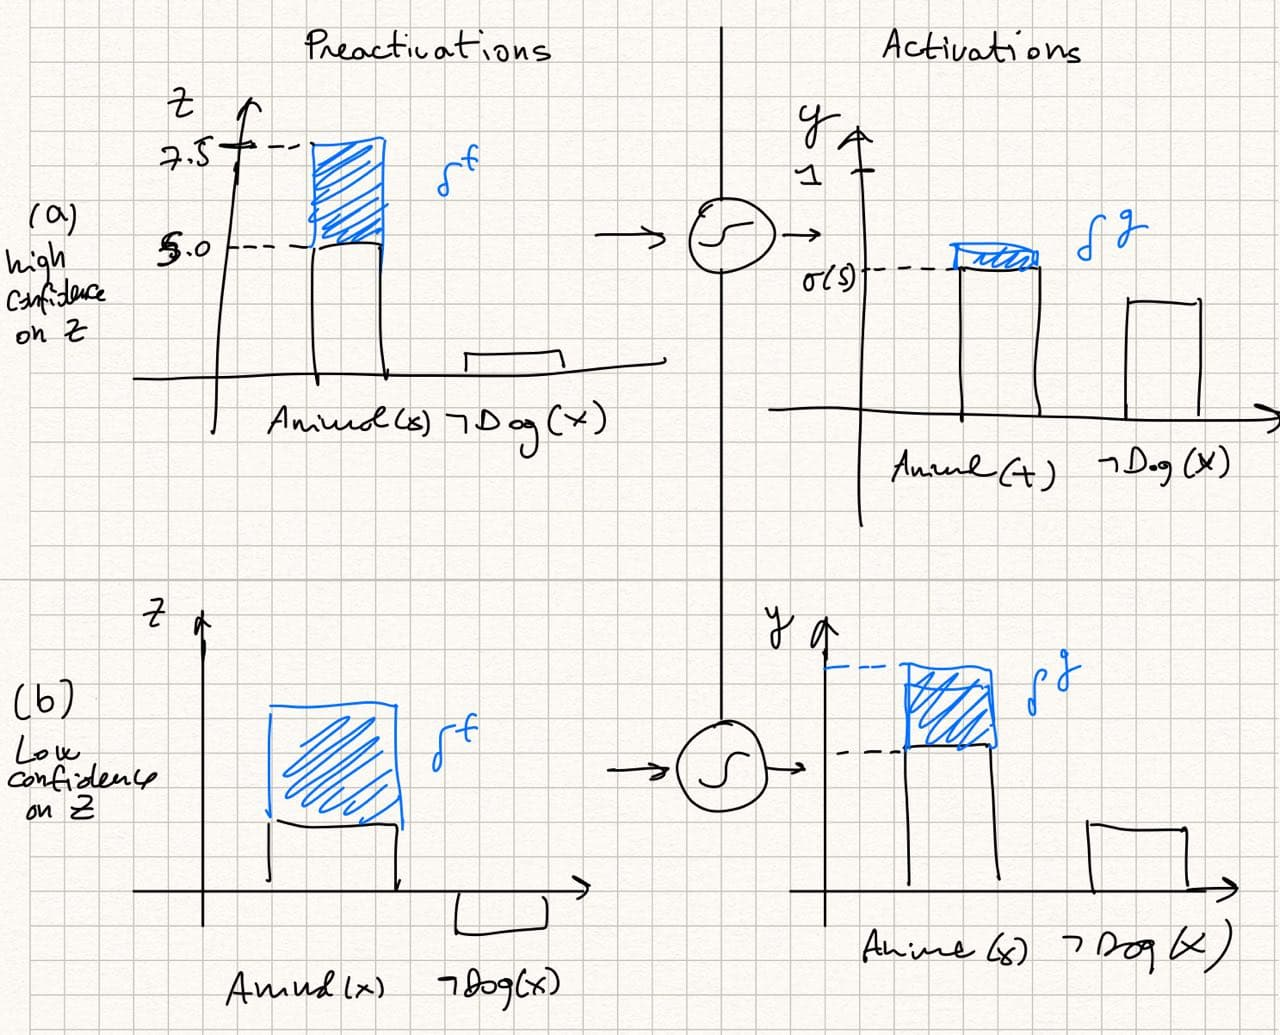
\includegraphics[width=0.8\textwidth]{figures/preac_deltas_example.jpg}
	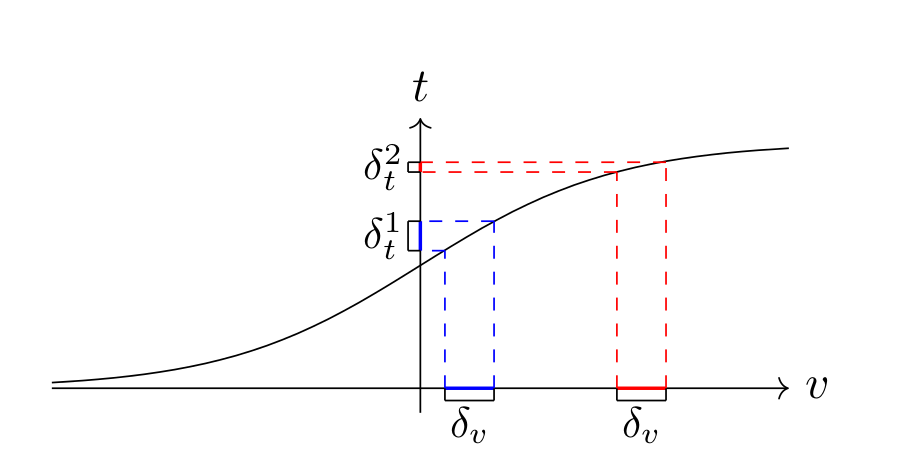
\includegraphics[width=0.5\textwidth]{figures/sigmoid_shape_example.png}
	%TODO: refine this caption
	\caption{This image illustrates the actual deltas produced by KENN, which are the $\delta^f$, opposed to the actual delta produced on the activations, which is $\delta^g$. As we said, $\delta^g$ is not produced directly by the model but it is indirectly \textit{induced} by the application of $\delta^f$ on the preactivations. This also illustrates how, thanks to the shape of the sigmoid activation function, the same delta on the preactivation produces a different delta at the activations level: the closer the preactivations to zero, the highest the modification on the final predictions. }
	\label{fig:preacs_deltas_example}
\end{figure}

As we already mentioned, the minimal TBF directly modeled by KENN is the one we called $\delta^f(z)$. From its definition, we know that the magnitude of the produced delta is determined by the definition of $f$. One of the most important features of KENN is that, by design, it learns to give the proper \textit{importance} to each clause in the base knowledge: this precise feature of the model gives also a way to find such function $f$. Specifically, for each clause $c$ a learnable parameter $w_c$ is defined so that the produced delta for $c$ is:

\begin{equation*}
\delta^{w_c}(z)_i = 
\begin{cases}
w_c \quad &\text{if } i = \arg\max_{j=1}^nz_j \\
0 \quad &\text{otherwise.}
\end{cases}
\end{equation*}

From this definition it's now clear that the function $f$ we were looking for is not actually the same for all the clauses in the base knowledge, but it is defined for each different clause and it's equal to the constant function $f_c(z) = w_c, \quad w_c \in \left[0, \infty\right]$. 
There is one last problem: while it's true that the function $\delta^{w_c}$ is a minimal TBF, the implementation of this kind of functions inside a NN is unfeasible since they are not differentiable. For this reason KENN uses a soft approximation of $\delta^{w_c}$, defined as:

\begin{equation}
\delta_s^{w_c}(z)_i = w_c \cdot \operatorname{softmax}(z)_i = w_c \cdot \frac{e^{z_i}}{\sum_{j=1}^ne^{z_j}}.
\label{eq:soft_approx_delta}
\end{equation}

There are still, however, some steps to describe in order to fully understand how KENN produces a vector of deltas. Recall our notation: we defined with $y \in \mathbb{R}^m$ the vector of predictions from the NN. Specifically, we now define with $y_A$ the truth value relative to $A$, where $A$ is a generic predicate of our language. We also define $z_A=\sigma^{-1}(y_A)$. Now, we note that equation (\ref{eq:soft_approx_delta}), tells us that the produced $\delta$ is always $m$-dimensional, where $m$ is the number of output classes. This however is not desirable: in fact, in general, not all the clauses in our base knowledge contain all the predicates of our language. For example, given $\mathcal{P}=\{A,B,C\}$, the clause $c = A \vee \neg B$ contains only two of the three predicates in the language. Therefore, we would like this specific clause to not modify in any way $z_C$. Another problem is that we don't know how to express the preactivation of a negated literal, i.e. we don't know how to derive $z_{\neg A}$ from $z_A$. In fact, recall that in equation (\ref{eq:lukasiewicz}) we defined the interpretation of a negated predicate, where we knew that the truth values were well defined in the interval $\left[0,1\right]$. Now we are dealing with preactivations, which cannot be considered truth values in the Fuzzy Logic theoretical framework. However, this problem can be easily solved by exploiting the following property of the sigmoid activation function:

\begin{equation*}
1 - \sigma(x) = \sigma(-x).
\end{equation*}

Now it's easy to see that, since $y_{\neg A} = 1 - y_A$, we can define:

\begin{equation*}
z_{\neg A} = -z_A.
\end{equation*}

Notice that we are not introducing any new concepts: instead we are just redefining quantities that were already mentioned at the activation level, to the preactivation level. %TODO Maybe remove this sentence
We finally define $z_c = \left(z_{l_1}, \dots, z_{l_k}\right)$ for every clause $c := \bigvee_{i=1}^k l_i$ of the knowledge. We refer to the process of transforming from $z$ to $z_c$ as the \textit{selection} step. This new vector contains only the preactivations of literals present in $c$, and is the one that we actually want to use to produce the delta relative to clause $c$. Now, let $\mathcal{K}$ be the set of clauses in our knowledge, and $\{w_c\}_{c\in\mathcal{K}}$ their corresponding weights. For every clause $c\in \mathcal{K}$ we want to obtain a new delta, namely $\delta^c \in \mathbb{R}^m$, which contains one value for each predicate in the clause and is defined as follows:

\begin{equation}
\delta_{A}^{c}= \begin{cases}\delta_{s}^{w_{c}}\left(z_{c}\right)_{A} & \text { if } A \in c \\ -\delta_{s}^{w_{c}}\left(z_{c}\right)_{\neg A} & \text { if } \neg A \in c \\ 0 & \text { Otherwise }\end{cases}, \quad \forall A \in \mathcal{K}
\end{equation}

This newly defined delta, $\delta^c$, will be the delta obtained from clause $c$ and will be summed to $z$ to obtain the updated prediction. More specifically:

$$y' = \sigma(z + \delta^c)$$

\begin{figure}[h!]
	\centering
	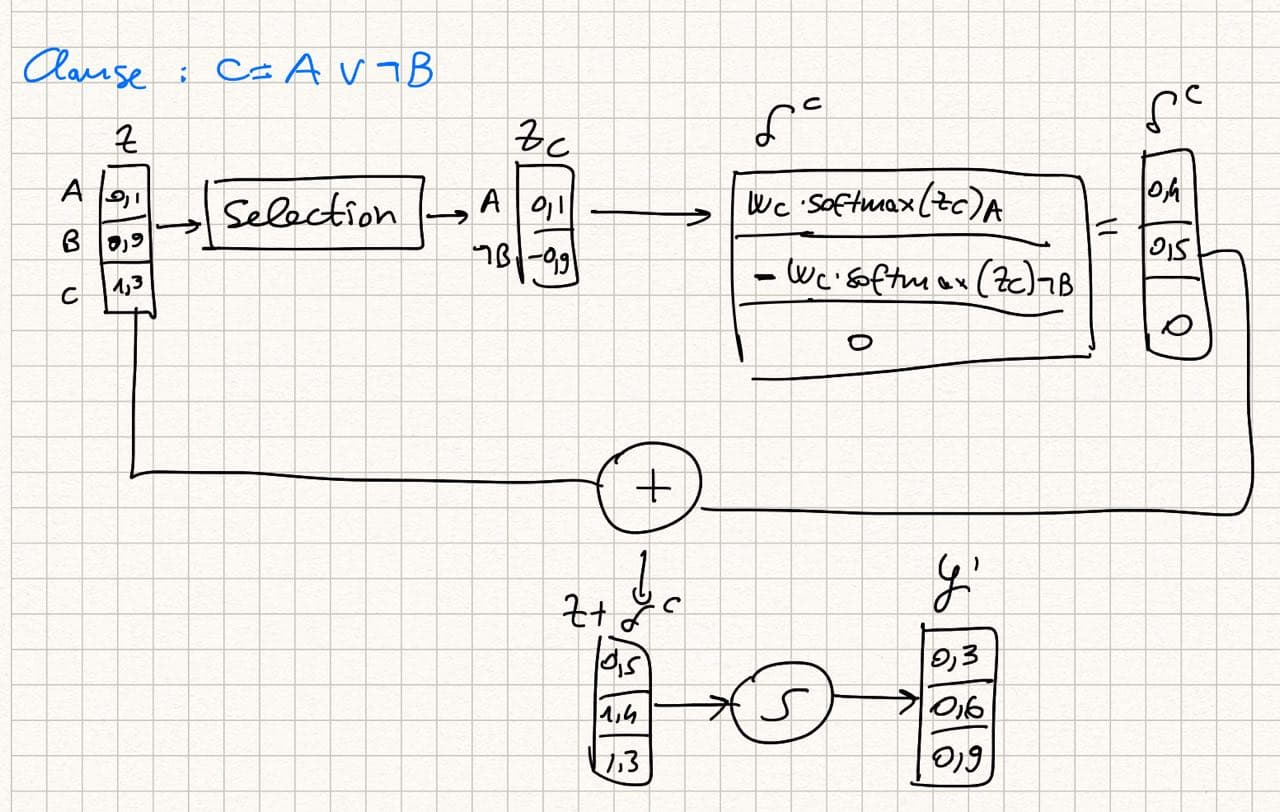
\includegraphics[width=0.8\textwidth]{figures/delta_single_clause.png}
	\caption{Summary of all the steps needed to produce $\delta^c$, the vector of deltas derived from a single clause. We refer to this process as \textit{clause enhancement}.}
	\label{fig:delta_single_clause}
\end{figure}


\subsection{Increasing the satisfaction of the Knowledge}
In the previous section we found out how KENN produces a vector of changes $\delta$ to be applied to the original NN predictions, but only considering a single clause. In the cases where the knowledge is constituted only by a single clause, we would already know how KENN works, but in real applications a higher number of logical rules will be desirable. Therefore, the next and final problem is to understand how KENN takes all the deltas from all the clauses and produces a single vector of changes. This particular step of aggregation is critical, as it constitutes one of the best features of KENN, but at the same time one of its bigger inaccuracies. This is because, to aggregate the contributions from all the clauses $c \in \mathcal{K}$, KENN just sums the contributions. Specifically, the final prediction is defined as follows:

\begin{equation*}
y'=\sigma(z + \sum_{c\in\mathcal{K}}\delta^c).
\end{equation*}
This particular choice makes KENN really fast at inference and learning time, increasing scalability. At the same time, though, this makes the risk of inconsistencies higher. For example, the same predicate can appear negated in one clause, and not negated in another clause: in this way the delta for the first one will be negative while it will be positive for the second one. In this way, the two delta may cancel out rendering KENN less useful.


\section{KENN Architecture}

